\documentclass[twocolumn,amsmath,amssymb,aps]{revtex4}
\usepackage{graphicx}% Include figure files
\usepackage{dcolumn}% Align table columns on decimal point
\usepackage{bm}% bold math
\usepackage{color, subfigure}

\begin{document}
\title{An Overview of the Belousov-Zhabotinsky Chemical Oscillations}%
\author{Huan Q, Bui}\email{hqbui21@colby.edu}
\affiliation{Departent of Physics and Astronomy, Colby College.}
\date{\today}
\begin{abstract}
This paper reviews the Belousov-Zhabotinsky reaction and the Oregonator. Specifically, we explore how the Oregonator captures the characteristic behaviors of the Belousov-Zhabotinsky reaction through the existence of the limit cycle and excitability. We also briefly discuss the history and significance of the Belousov-Zhabotinsky reaction. 
\end{abstract}
\maketitle




\section{Introduction}
The Belousov-Zhabotinsky (BZ) reaction, named after Soviet chemists Boris Belousov (1893 - 1970) and Anatol Zhabotinsky (1938 - 2007), are an important example of a large class of chemical oscillators. The reaction was first discovered by Belousov in 1951 in his attempt to mimic glycolysis, an oscillatory biochemical process in which glucose is metabolized. Using a mixture of potassium bromate, cerium(IV), sulfate, malonic acid, and citric acid in dilute sulfuric acid at appropriate proportions, Belousov found that the solution color spontaneously oscillated between clear and yellow rather than reaching an equilibrium state. This behavior was so peculiar that Belousov's contemporaries refused to publish his results, citing the apparent violation of the second law of thermodynamics, which states that a system must attain a preferred equilibrium state \cite{ball1999self}. Belousov ultimately managed to publish his results, but in a less reputed and non-peer-reviewed journal. The reaction was further studied in 1961 by Zhabotinsky and only gained popularity in the Western scientific community after a conference in Prague in 1968\cite{doi:10.1021/ed061p661}.

Today, the BZ reaction remains popular among academics. It is a prime example for a nonlinear system in a thermodynamic  non-equilibrium which also exhibits excitability and oscillatory behaviors. Following its emergence into the scientific canon, mathematical models for the reaction also attract significant interest. The most notable examples of these models are the \textit{Brusselator}, proposed by Ilya Prigogine and his collaborators at the Université Libre de Bruxelles, and the \textit{Oregonator}, proposed by Richard Field and Richard M. Noyes at the University of Oregon. While the Brusselator helped motivate interest in chemical pattern formation, it does not model a realistic BZ reaction. The Oregonator, on the other hand, captures many aspects of a true chemical oscillator including limit cycle dynamics and excitability.

When taking place in an appropriate geometry, the BZ reaction becomes a \textit{reaction-diffusion system} which gives rise to pattern-forming \textit{chemical waves} \cite{ball1999self}. Unlike sound waves or electromagnetic radiation, however, these waves do not interfere the same way sound of electromagnetic waves do, i.e., they do not obey the principles of superposition. In a different setting, the BZ reaction manifests as oscillations. This papers focuses mainly on the latter behavior through an overview of the Oregonator.

\section{The Oregonator}
The Oregonator is a system of two coupled ordinary differential equations \cite{doi:10.1063/1.1681288}:
\begin{eqnarray}
\epsilon \dot{U} &=& U(1-U) - fV(U-q)/(U+q) \\
\dot{V} &=&  U-V
\end{eqnarray}
where $U,V$ represent the concentrations of HBrO$_2$ and Ce$^{4+}$, respectively. The Oregonator provides a realistic mechanism linking limit cycle dynamics to a real-world chemical oscillator. The equilibrium concentrations are attained whenever $\dot{U} = \dot{V} = 0$. These solutions are given by the following expressions:
\begin{eqnarray}
U_{\text{eq}} &=& \frac{1}{2}\left[1-q-f + \sqrt{(1-q-f)^2 + 4q(1+f)}\right]\nonumber \\ 
V_{\text{eq}} &=& U_{\text{eq}}. 
\end{eqnarray}
One finds this equilibrium solution by intersecting the nullclines $\dot{U} = 0$ and $\dot{V} = 0$:
\begin{eqnarray} 
V &=& \frac{U(1-U)(U+q)}{f(U-q)}\\
V &=&U 
\end{eqnarray}
It is clear that the first nullcline depends only on the parameters $f$ and $q$, and the second nullcline is independent of all model parameters. For the rest of this paper, we will assume $q$ is fixed unless stated otherwise. As we will see later, by varying $f$, the model exhibits markedly different behaviors. 

\subsection{Limit Cycle}
The Oregonator captures the oscillatory behavior of the BZ reaction through the existence of the \textit{limit cycle} for certain combinations of the parameters $f,q$, and $\epsilon$. A limit cycle is an attractor, i.e., a solution for the Oregonator towards which the system tends to evolve in the large-time limit. The limit cycle shows up as a closed trajectory in phase space. In the presence of a limit cycle, any out-of-equilibrium state of the system converges to no fixed point. 

\begin{figure}[!htb]
	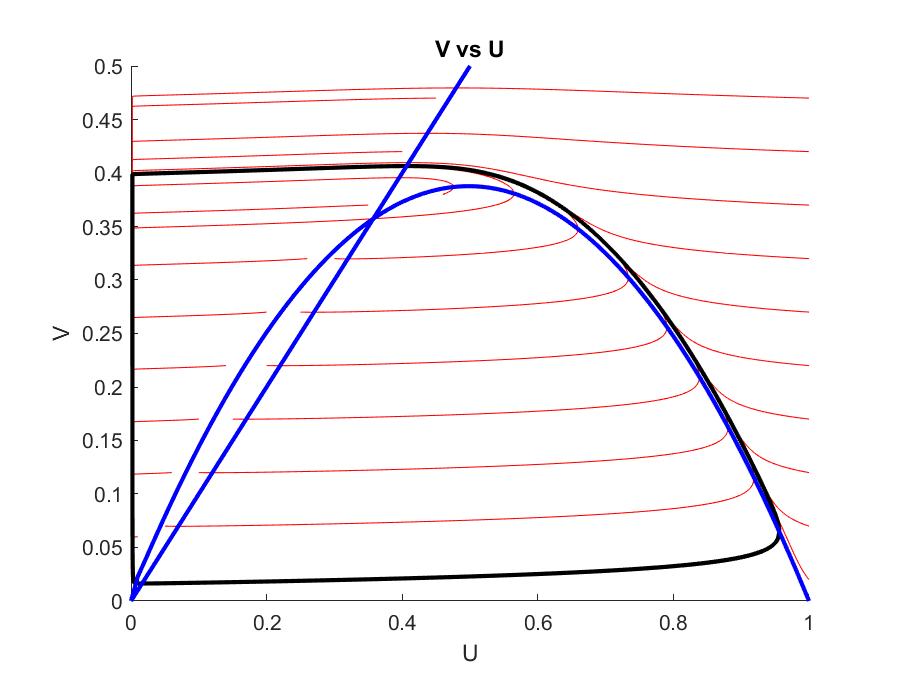
\includegraphics[scale=0.5]{limit_cycle_f_065_e_1e-2.eps}
	\caption{Limit cycle (black) and nullclines (blue), for $f = 0.65, \epsilon = 10^{-2}, q = 0.002$. All trajectories (except for the equilibrium trajectory) converge to the limit cycle, including points near the equilibrium solution. Points to left of the $V=U$ nullcline converge the limit cycle from the right, and vice versa. The system does not converge to  a fixed point.}
	\label{fig:LC}
\end{figure}

Figure \ref{fig:LC} shows the phase portrait of the system at $f = 0.65, \epsilon = 10^{-2}$, and $q = 0.002$. All phase trajectories, except for the equilibrium trajectory at $U_{\text{eq}} = V_{\text{eq}} = 0.3572$ (which is the intersection between two nullclines highlighted in blue), converge to the counter-clockwise limit cycle highlighted in black. All trajectories which begin below the parabolic nullcline first evolve towards an increase in $U$, while those above the parabolic nullcline first evolve towards a depletion in $U$. Figure \ref{fig:UVTime} shows how the system evolves following the initial condition given by $U_0 = 0.2, V_0 = 0.26$, which is above the parabolic nullcline. 


\begin{figure}[!htb]
	\centering
	\includegraphics[scale=0.5]{UV_Time.eps}
	\caption{Oscillations in concentration of $U,V$ in time is the presence of a limit cycle. The system evolves from the initial condition $U_0 = 0.2, V_0 = 0.26$}
	\label{fig:UVTime}
\end{figure}


Just to emphasize the fact that \textit{all} trajectories, no matter how close to the equilibrium solution, converge the limit cycle, we consider the initial condition $U_0 = U_{\text{eq}} + 10^{-7}$ and $V_0 = V_{\text{eq}} + 4\times 10^{-8}$. This initial condition corresponds to a very small perturbation from the equilibrium solution. Figure \ref{fig:Perturbed} shows that the system evolves into oscillations. Because of this property, any state of a system which obey the Oregonator description with a limit cycle almost always goes into oscillations.

\begin{figure}[!htb]
	\centering
	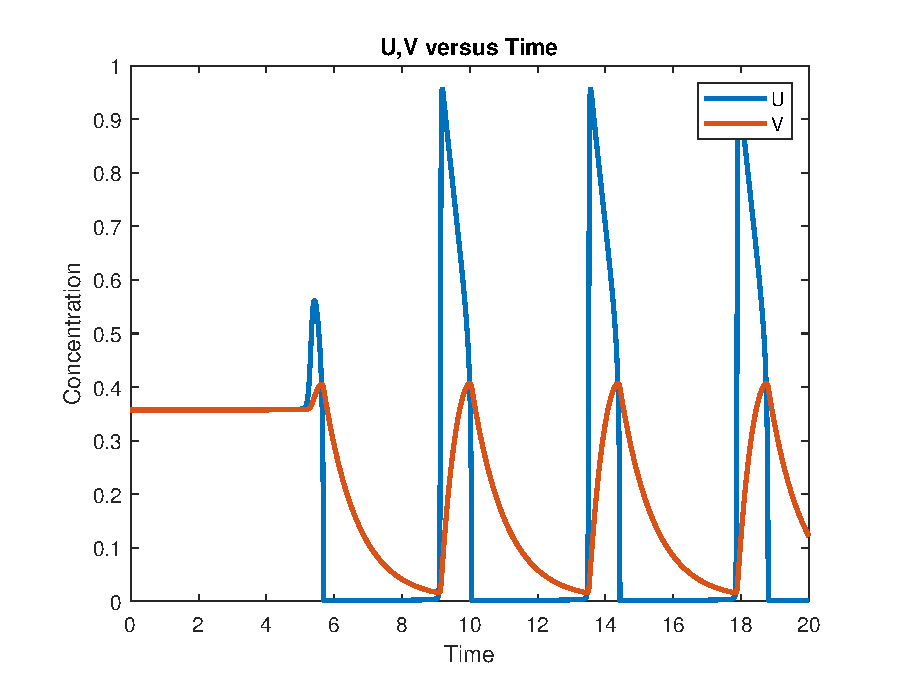
\includegraphics[scale=0.5]{perturbed.eps}
	\caption{Oscillations in concentration of $U,V$ in time is the presence of a limit cycle. The system evolves from the initial condition $U_0 = U_{\text{eq}} + 10^{-7}, V_0 = V_{\text{eq}} + 4\times 10^{-8}$}
	\label{fig:Perturbed}
\end{figure}



\subsection{Hopf Bifurcation}

The Hopf bifurcation, in the context of this paper, is a critical point in the parameter space $(f,q,\epsilon)$ at which the limit cycle appears. So far, we have assumed that $f = 0.65, \epsilon = 10^{-2}$, and $q = 0.002$, at which point the model has a limit cycle shown in Figure \ref{fig:LC}. For simplicity, let us assume that $q,\epsilon$ are fixed. By varying $f$, we will see that the limit cycle disappears when $f$ is too small or too large. For example, consider the case where $f=2.45$. Figure \ref{fig:hopf1} shows that solutions now converge to fixed point. $f$ is too large, and the limit cycle no longer exists.
\begin{figure}[!htb]
	\centering
	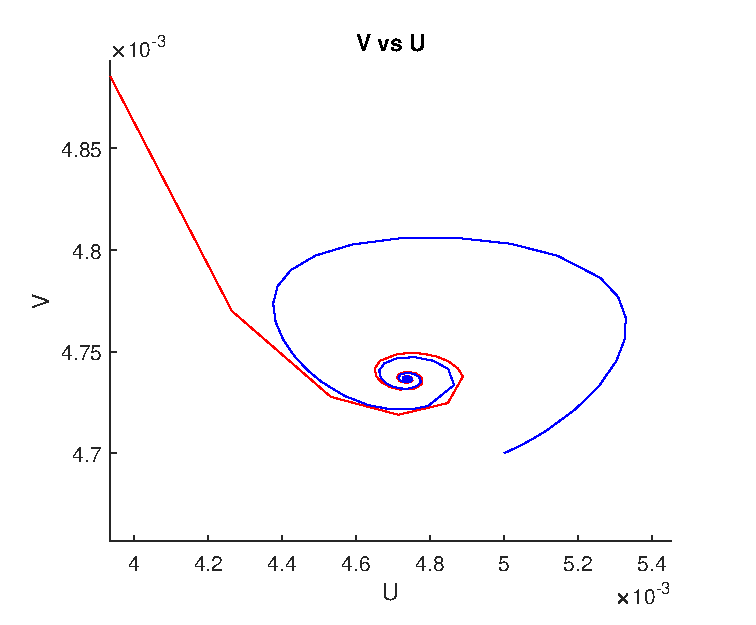
\includegraphics[scale=0.6]{hopf1.eps}
	\caption{$f = 2.45$. Solutions converge to a stable fixed point: the red line denotes initial condition $U_0 =V_0 = 4\times 10^{-3}$; the black line denotes the initial condition $U_0 = 5\times 10^{-3}, V_0 = 4.7 \times 10^{-3}$.}
	\label{fig:hopf1}
\end{figure}


The limit cycle also disappears when $f$ is too small. Consider the case where $f = 0.505$. The initial condition $U_0 = V_0 = 0.6$ evolves and spirals towards the fixed point shown in Figure \ref{fig:hopf2}.
\begin{figure}[!htb]
	\centering
	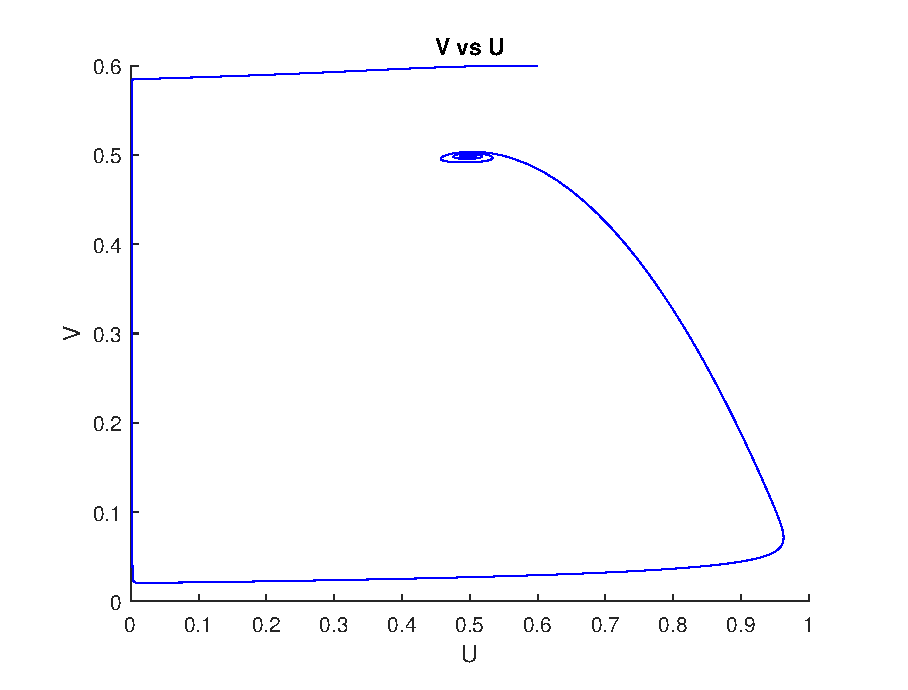
\includegraphics[scale=0.6]{hopf2.eps}
	\caption{$f = 0.505$. Solutions converge to a stable fixed point: the red line denotes initial condition $U_0 =V_0 = 4\times 10^{-3}$; the black line denotes the initial condition $U_0 = 5\times 10^{-3}, V_0 = 4.7 \times 10^{-3}$.}
	\label{fig:hopf2}
\end{figure}
To see how the system reaches a stable equilibrium in the large-time limit, we can also look at how $U$ evolves in time in Figure \ref{fig:UEvolves}.
\begin{figure}[!htb]
	\centering
	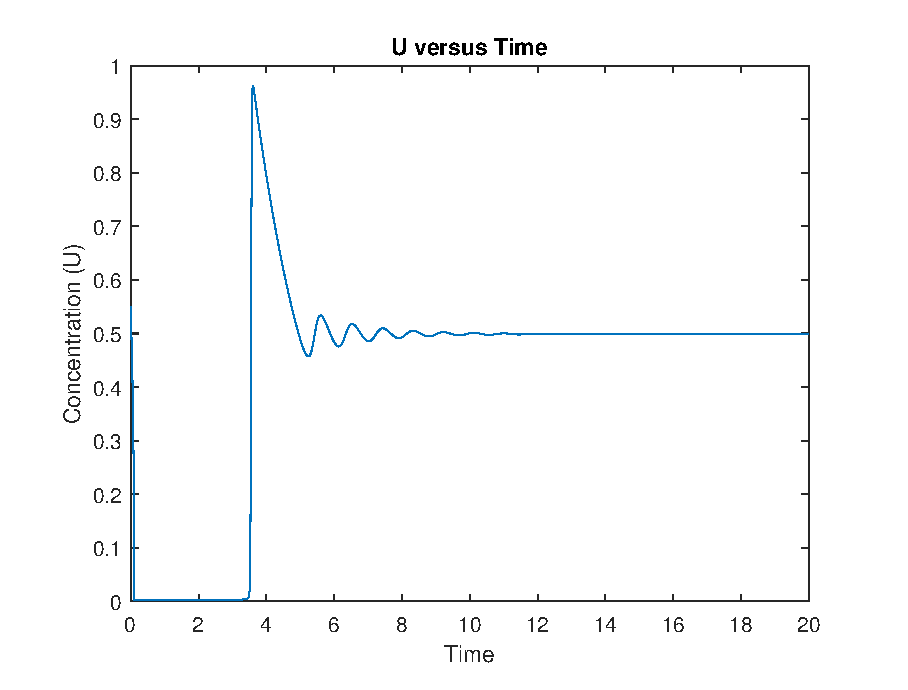
\includegraphics[scale=0.6]{hopf2_time.eps}
	\caption{$f = 0.505$. The concentration in $U$ approaches a stable fixed point.}
	\label{fig:UEvolves}
\end{figure}

It is possible to map out all the combinations of $(f,q,\epsilon)$ for which the Oregonator has a limit cycle. This can be done through stability analysis of the Oregonator as well as careful numerics. For the sake of simplicity, however, we will not cover how this is done.


The Hopf bifurcation is not unique to the Oregonator. Not surprisingly, this bifurcation also appears in the BZ reaction, as well as in the Brusselator, the Hodgkin-Huxley model, and the FitzHugh-Nagumo model. In fact, these models are closely related and share a number of common characteristics including \textit{excitability}, which we will cover in the next subsection.


\subsection{Excitability}
An excitable system is a nonlinear system which can be characterized by the following two properties. For small perturbations away from the equilibrium state, the system responses monotonically with the perturbations.  However, when the perturbation is sufficiently large (beyond some threshold), the system becomes \textit{excited} and undergoes a markedly different, often more extreme, trajectory.  

In this subsection we shall see that the Oregonator, under appropriate conditions, can be an excitable system. From the preceding subsection, we have seen that the Oregonator can exhibit limit cycles for certain values of $(f,q,\epsilon)$. When a limit cycle exists, all solutions except for the equilibrium converge to the limit cycle, and for any perturbation from the equilibrium state the system eventually behaves the same way. It is thus clear that the system cannot be excitable in the presence of a limit cycle. 

This leaves the only other possibility: that the system is excitable when no limit cycle exists. It remains for us to find evidence of excitability. To this end, we must first remove the limit cycle by considering the combination $(f,q,\epsilon) = (3,0.002, 0.01)$. The Oregonator indeed exhibits no limit cycle, according to the phase portrait shown in Figure \ref{fig:NoLimitCycle}. Even though solutions might follow a similar trajectory as in the case with the limit cycles, since these trajectories are not closed curves, they are not limit cycles. Upon careful inspection, one finds that all trajectories actually converge to the equilibrium point $(0.004,0.004)$ of the model. 
\begin{figure}[!htb]
	\centering
	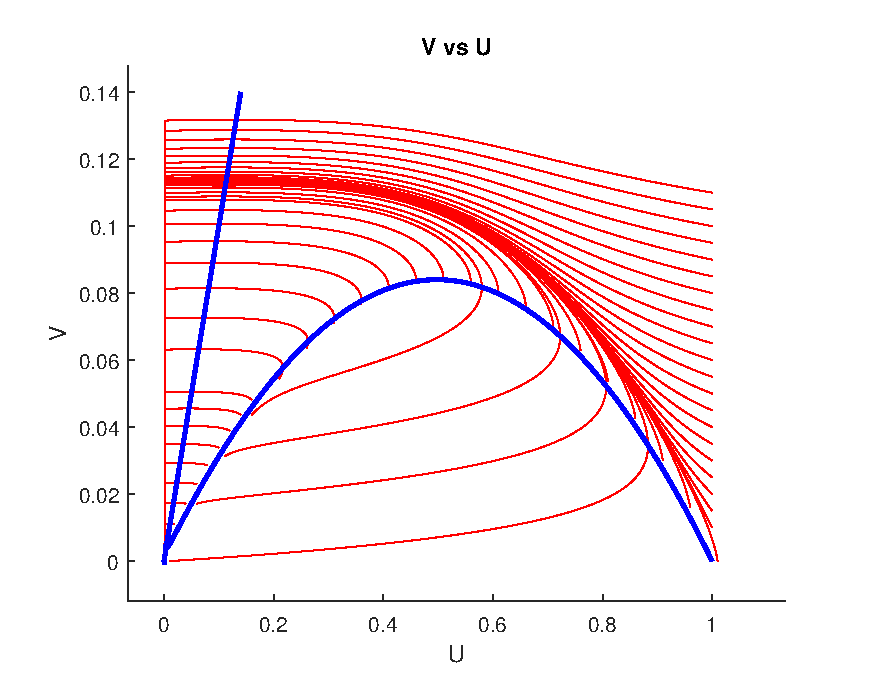
\includegraphics[scale=0.6]{no_limit_cycle.eps}
	\caption{No limit cycle present when $(f,q,\epsilon) = (3,0.002, 0.01)$. All solutions converge to the equilibrium point $(0.004,0.004)$. No phase trajectory is a closed curve.}
	\label{fig:NoLimitCycle}
\end{figure}

We can now find evidence of excitability in the system. To this end, we consider how the system evolves from a neighborhood around the equilibrium solution. Particularly, we consider the set of initial conditions of the form $(U_0, V_0 - \delta)$ where $\delta \in [0, 3.7\times 10^{-4}]$. Figure \ref{fig:Excite1} shows the phase trajectories associated with these initial conditions, with the nullclines highlighted in blue. The equilibrium is again the intersection of the two nullclines. Figures \ref{fig:Excite1} and \ref{fig:Excite2} combined show how the system evolves under this set of initial conditions. It is clear that the system possesses two characteristically distinctive behaviors, despite having very similar initial conditions:
\begin{itemize}
	\item For small perturbations from the equilibrium, the system \textit{immediately} returns to the equilibrium state (appearing as small convex curves above the parabolic nullcline in Figure \ref{fig:Excite1}). In this case we say that the system is not excited.
	\item When the perturbation is sufficiently large, the system undergoes a markedly different trajectory than an immediate return to the equilibrium state (appearing as D-shaped curves in Figure \ref{fig:Excite2}). In this case we say that the system is excited.
\end{itemize}
\begin{figure}[!htb]
	\centering
	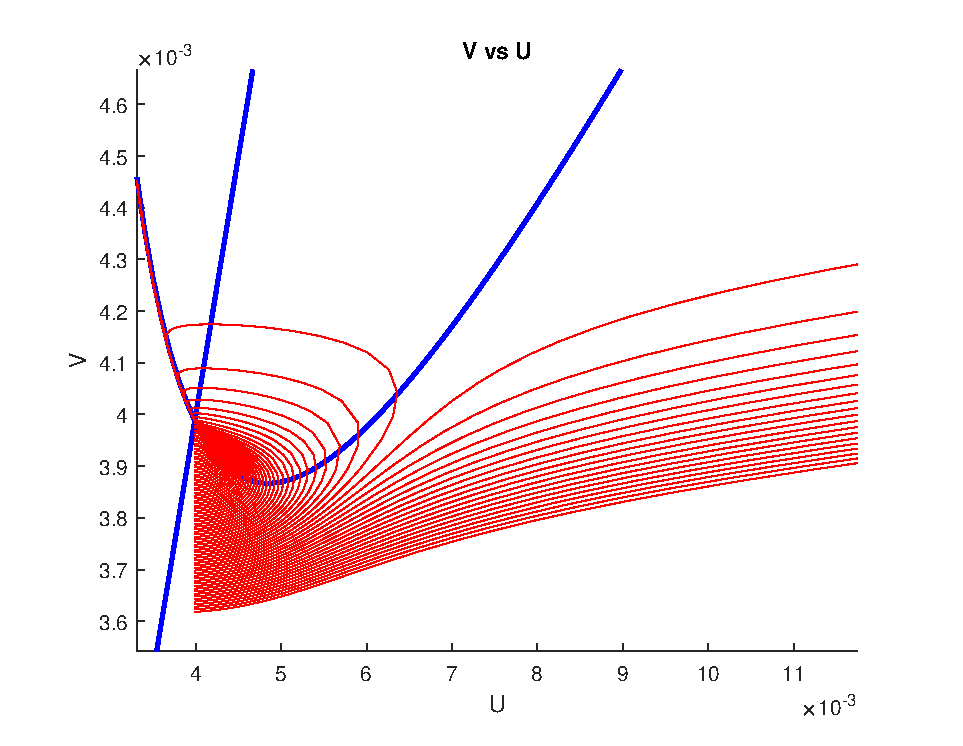
\includegraphics[scale=0.55]{excite_1.eps}
	\caption{How the system evolves under various initial conditions. Here $(f,q,\epsilon) = (3,0.002, 0.01)$. The region of interest is a small neighborhood of the origin.}
	\label{fig:Excite1}
\end{figure}
\begin{figure}[!htb]
	\centering
	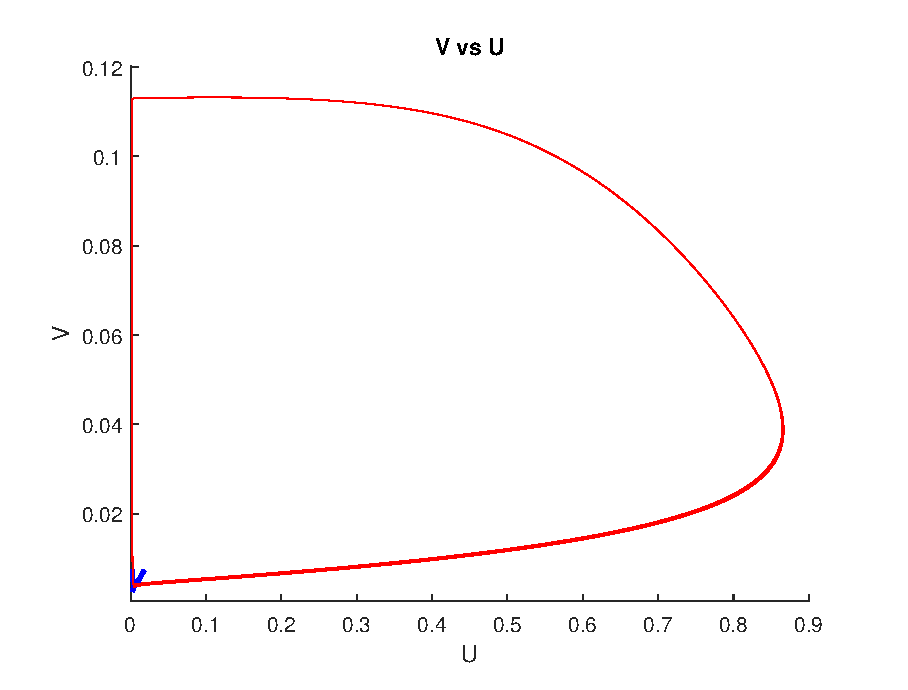
\includegraphics[scale=0.5]{excite_22.eps}
	\caption{How the system evolves under the same set of initial conditions. The region of interest now contains all phase trajectories generated from these initial conditions. The blue line in the bottom left corner is the linear nullcline in Figure \ref{fig:Excite1}.}
	\label{fig:Excite2}
\end{figure}

Figure \ref{fig:Excite3} further illustrates the transition from an unexcited to an excited state of the system. When the perturbation is small, the maximum in $U$ remains in a neighborhood of the initial condition (and the equilibrium value). However, when the perturbation in $V$ exceeds a threshold value between $2.5 \times 10^{-4}$ and $3 \times 10^{-4}$, the concentration $U$ possesses a large spike as a function of time. 


\begin{figure}[!htb]
	\centering
	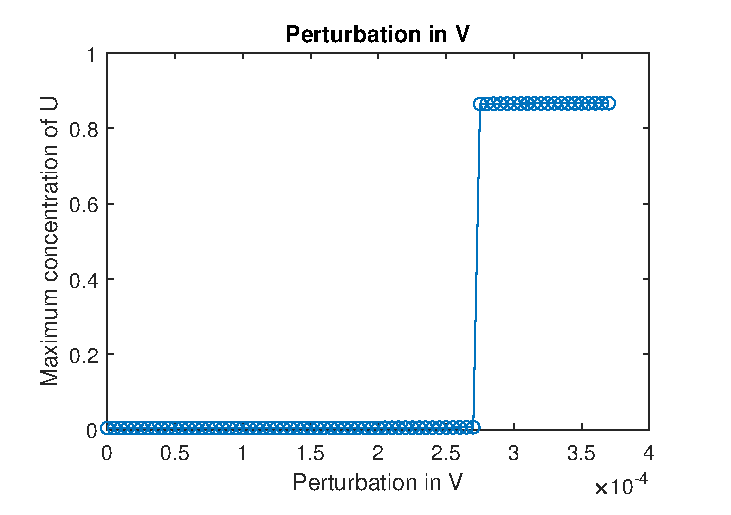
\includegraphics[scale=0.6]{excite_2.eps}
	\caption{Plot of the maxima in $V$ at various perturbation amplitudes. Perturbations beyond a threshold value between $2.5\times 10^{-4}$ and $3\times 10^{-4}$ excite the system.}
	\label{fig:Excite3}
\end{figure}


\begin{figure}[!htb]
	\centering
	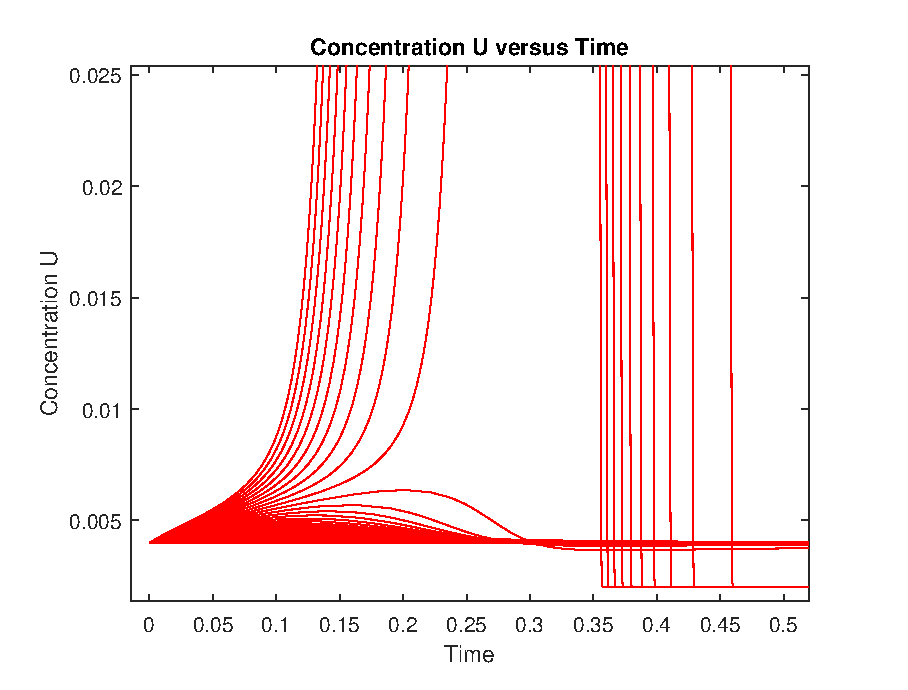
\includegraphics[scale=0.5]{UvTime.eps}
	\caption{Concentration $U$ as a function of time. For perturbations beyond the threshold value, $U$ has a large spike and eventually returns to the equilibrium value.}
	\label{fig:Excite4}
\end{figure}





\section{Discussions}


\subsection{BZ reaction as real-world manifestations of the limit cycle and excitability of the Oregonator}

The Oregonator captures not only the oscillatory behavior through the existence of the limit cycle but also the excitability of the BZ reaction. These two phenomena appear under different experimental settings. BZ oscillations occur when the reactants are constantly mixed in order to maintain uniform chemical concentrations throughout the medium in which the reaction takes place.  Figure \ref{fig:Osc} shows a flask containing the reaction at two different points in time, and Figure \ref{fig:osc-time} shows how the color of the solution oscillates in time. We notice that these oscillations occur at regular intervals, but are not strictly periodic. 
\begin{figure}
	\centering
	\subfigure[]{\includegraphics[scale=0.08]{osc0}}
	\subfigure[]{\includegraphics[scale=0.08]{osc1}}
	\caption{The solution oscillates between the two states (a) and (b). Constant stirring is required.}
	\label{fig:Osc}
\end{figure}


\begin{figure}[!htb]
	\centering
	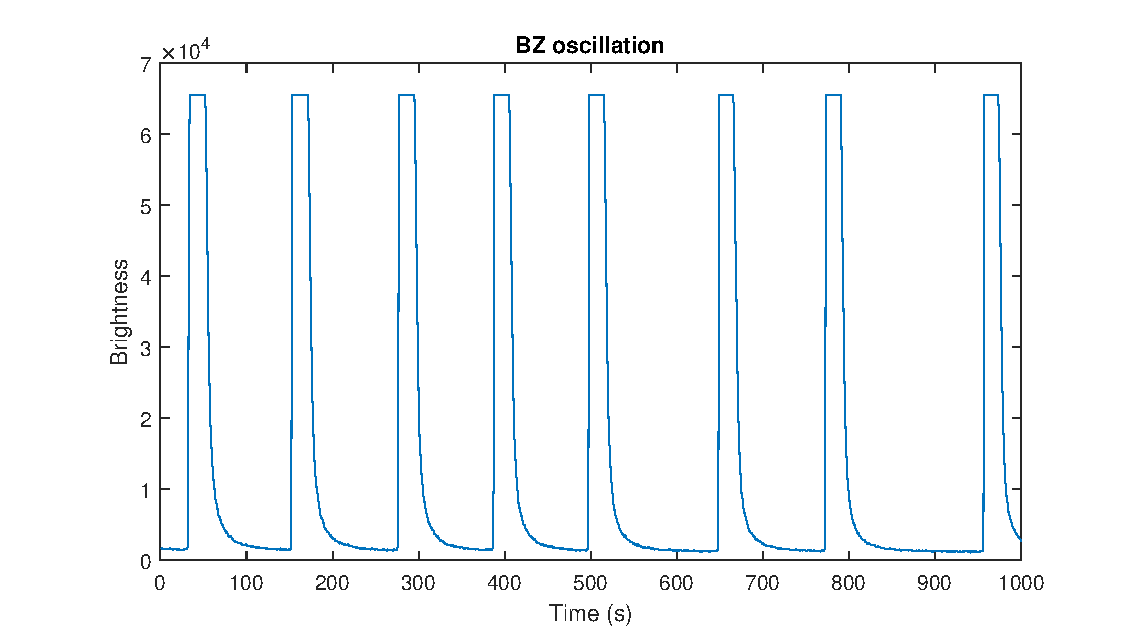
\includegraphics[scale=0.45]{osc-lab}
	\caption{Brightness of the solution in Figure \ref{fig:Osc} as a function of time. Notice that these oscillations do not occur with a constant period.}
	\label{fig:osc-time}
\end{figure}


In the absence of vigorous stirring, diffusion becomes important, and the system becomes an excitable, pattern-forming, \textit{reaction-diffusion system}. Figure \ref{fig:Pattern} shows a typical pattern and how it evolves in time. 


\begin{figure}
	\centering
	\vspace{+15pt}
	\subfigure[]{\includegraphics[scale=0.08]{pattern0}}
	\subfigure[]{\includegraphics[scale=0.08]{pattern1}}
	\caption{Pattern formation due to the BZ reaction.}
	\label{fig:Pattern}
\end{figure}


Here, the reaction generates traveling chemical waves. Unlike sound or electromagnetic waves, these waves do not necessarily obey the principle of superposition. For instance, two BZ wavefronts annihilate each other when they meet. The pattern-forming property is due to the interplay between reaction and diffusion. Turing patterns are a classical example of patterns formed through such a process. 





\subsection{BZ reaction in Non-equilibrium thermodynamics}

The second law of thermodynamics states that a system must tend towards higher entropy, i.e., coffee never unstirs itself into water, sugar, and coffee beans. This law guarantees for every chemical reaction a preferred direction towards a preferred equilibrium state. The BZ reaction, despite having seemingly perpetual oscillations, is no exception. The oscillations eventually diminish and vanish. Given sufficient time, the system will reach a stable equilibrium state at which its total entropy is higher than that before the reaction took place. 

In spite of this, the BZ reaction is still interesting because of its peculiar path towards equilibrium. Likewise, many fascinating processes, such as the formation of life or the creation of societies, take place in out-of-equilibrium states. \cite{ball1999self}




\begin{acknowledgments}
I thank Professor McCoy for introducing HQB to this topic, his guidance through this project, and the image data for the BZ reaction. I also thank Shannon Gray and Emily Padula for the helpful discussions and the original version of the BZ lab MATLAB code.  
\end{acknowledgments}


\bibliography{paper1}


\end{document}